\documentclass{standalone}
\usepackage{tikzducks}

\colorlet{horse}{white!90!black!90!brown}

\begin{document}

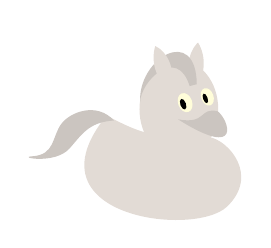
\begin{tikzpicture}[xscale=-1]

  \begin{scope}[yshift=-6]
    \clip[rotate=-5] (0.68,2.38) ellipse (0.3 and 0.4);
    \fill[horse,rotate=-5](0.28,2.26)ellipse (0.3 and 0.4);
  \end{scope}
  \duck[
    body=horse,
    mohican=horse!90!black,
    horsetail,
    bill=horse!90!black
  ]
  \begin{scope}[yshift=-5,xshift=1]
    \clip[rotate=-5] (0.68,2.38) ellipse (0.3 and 0.4);
    \fill[horse,rotate=-5](1.06,2.2) ellipse (0.3 and 0.4);
  \end{scope}

\end{tikzpicture}

\end{document}